\documentclass[12pt,a4paper]{article}

% - TODO: extract citations from this paragraph to use elsewhere (why do we need AVs?)
    % - Although postulated that full autonomy could reduce human road fatalities by 90\% (due to the 90\% of deaths caused by human accident according to \ac{NHTSA}), this thought is derived under the assumption that SAE levels 4--5 of autonomy are accepted by regulatory bodies and the greater public, who present the greatest barrier to full autonomy \citep{a-review-and-analysis-of-lit-on-ad}. In order to overcome these hurdles, car makers will need to investigate novel features intended to reduce the technological opacity of current systems in order to enhance trust in the systems \citep{tech-opacity-predictability-sdc, importance-of-trust-on-adopting-av}. This problem becomes particularly challenging due to the difficulty of both (1) explaining the results of complex machine learning systems and (2) presenting the explanations to passengers in a way that improves trust without increasing cognitive load. Both of these roadblocks are well addressed in the literature, but not studied simultaneously.

% -------------------
% MARK: Packages
% -------------------

% import geometry package to update the document margins
\usepackage[margin=1in]{geometry}
% set the font to Times New Roman
% \usepackage{mathptmx}
% set the font to helvectica
\usepackage[scaled]{helvet}
\renewcommand\familydefault{\sfdefault}
% for type-setting
\usepackage{amsmath, amssymb, amsfonts, verbatim, pifont}
% for slashed out text
\usepackage[normalem]{ulem}
% for units and scientific notation
\usepackage[table]{xcolor}
\usepackage{siunitx}
% for references and URLs
\usepackage{hyperref, url}
% Natbib setup for author-year style
\usepackage{natbib}
 \bibpunct[, ]{(}{)}{,}{a}{}{,}%
 \def\bibfont{\small}%
 \def\bibsep{\smallskipamount}%
 \def\bibhang{24pt}%
 \def\newblock{\ }%
 \def\BIBand{and}%
% for graphics and figures
\usepackage{graphicx, subfig, tikz}
% a package for adding footnotes to figures
\usepackage[capposition=bottom]{floatrow}
% force figures to stay in their sections
\usepackage[section]{placeins}
% for tables
\usepackage{booktabs, longtable, tabularx}
\usepackage{multicol, multirow}
\usepackage{adjustbox}
\usepackage[flushleft]{threeparttable}
% a package for working with .csv data for tables
\usepackage{csvsimple}
% setup the algorithm package
% ruled: show bars around title and bar at bottom
% lined: show the line column on the left of the algorithm
% linesnumbered: print line numbers for each line
\usepackage[ruled,lined,linesnumbered]{algorithm2e}
\DontPrintSemicolon % don't print the semicolon that \; usually prints
% for acronyms
\usepackage[nolist]{acronym}
% import a nice author management package
\usepackage{authblk}
% import a package for double spacing
\usepackage{setspace}
\singlespacing
% for creating sub-figures within figures
% for combining multiple LaTeX files
\usepackage{subfiles}
% fix overfull hbox errors from oddities like using
% quotes (``foo'') and etc.
\usepackage{microtype}

% -------------------
% MARK: Debugging Packages (Comment out for final submission)
% -------------------

% import a debugging package to show the margin boxes
% \usepackage{showframe}
% put "Draft" as a watermark behind pages
% \usepackage{draftwatermark}
% \SetWatermarkLightness{0.95}

% -------------------
% MARK: Declarations
% -------------------

% setup captions for tables and figures
\captionsetup[table]{%
  labelfont={bf},
  name={Table},
  labelsep=colon,
  justification=raggedright,
  singlelinecheck=false}
\captionsetup[figure]{%
  labelfont={bf},
  name={Figure},
  labelsep=colon,
  justification=raggedright,
  singlelinecheck=false}

% set the graphics path to the img directory
\graphicspath{{img/}}

% a macro for making vectors, matrices, and tensors
\newcommand{\CKvector}[1]{\boldsymbol{\MakeLowercase{#1}}}
\newcommand{\CKmatrix}[1]{\boldsymbol{\MakeUppercase{#1}}}
\newcommand{\CKtensor}[1]{\mathbf{\MakeUppercase{#1}}}
% a macro for standard neural network theta
\newcommand{\NNtheta}{\boldsymbol{\theta}}
% operators for ArgMax and ArgMin
\DeclareMathOperator*{\argmax}{arg\,max}
\DeclareMathOperator*{\argmin}{arg\,min}

% a command for coloring a cell gray (siunitx friendly, i.e., {} enclosed)
\def\graycell{{\cellcolor[gray]{0.85}}}

% a command to run shell commands
% USAGE:
% \app@exe{<command>}
% where:
% - <command> is a shell command to run
%
\makeatletter
\def\app@exe{\immediate\write18}
\makeatother

% a command to include bibliographies from a directory.
% USAGE:
% \bibliographies{<directory>}
% where:
% - <directory> is a directory with .bib files to include
%
\makeatletter
\def\bibliographies#1{%
% compile all the bibliography files into a single references file
  \app@exe{find #1 -regex ".*bib" | xargs cat | egrep -v "(\%|^$|^\s*$)" > \jobname.references.bib}
% include the compiled bibliography file
  \bibliography{\jobname.references.bib}
}
\makeatother

% include the list of acronyms
% \begin{acronym}
% \acro{CV}
% \end{acronym}

% -----------------------------------------------------------------------------
% MARK: Algorithm stuff
% -----------------------------------------------------------------------------

% params
% \SetKwInOut{Objects}{$\CKmatrix{O}$}
% \SetKwInOut{Weights}{$\CKvector{w}$}

% -------------------
% MARK: Front Matter
% -------------------

% headers and footers
\usepackage{fancyhdr}
\setlength{\headheight}{15pt}
\pagestyle{fancy}
\lhead{KautenjaDSP}
\rhead{\itshape RackNES}
\cfoot{\thepage}

% -------------------
% MARK: Document
% -------------------

\begin{document}
% fancyhdr directive to remove headers from this title page
\thispagestyle{empty}
% center the title page contents
\topskip0pt
\vspace*{\fill}
\begin{center}

\includegraphics[width=0.8\textwidth]{RackNES-Logo}
\linebreak\linebreak\linebreak\linebreak
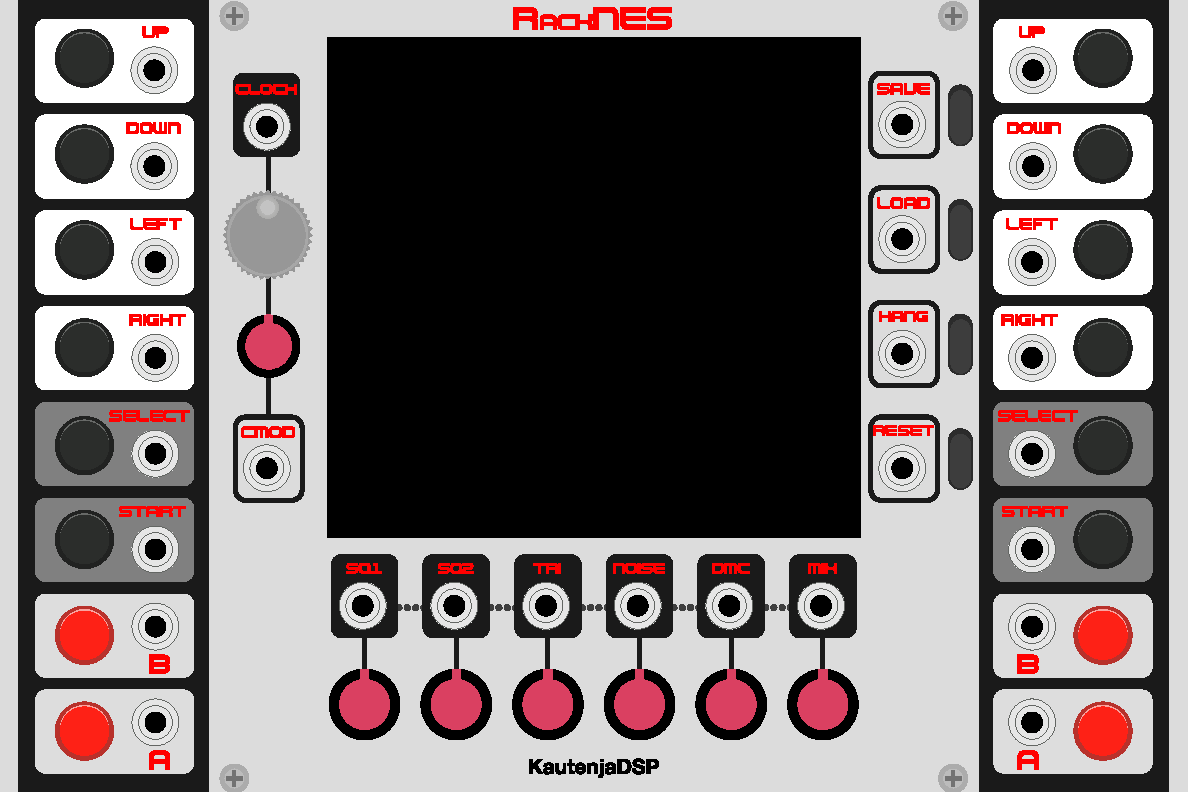
\includegraphics[width=0.8\textwidth]{RackNES-Module}
\linebreak\linebreak\linebreak\linebreak

\includegraphics[width=0.8\textwidth]{KautenjaDSP}
\end{center}
\vspace*{\fill}
\clearpage

% -------------------
% MARK: Overview
% -------------------

RackNES is a Nintendo Entertainment System (NES) emulator for VCV Rack with
control voltage inputs and outputs. RackNES offers several key features, namely,

\begin{itemize}
  \item \textbf{Clock Source:} Use NES frame-rate (FPS) as a clock source for downstream modules;
  \item \textbf{Clock Rate Modulation:} Control the clock rate of the NES with direct knob and CV;
  \item \textbf{NES Audio Output:} Sample audio from the NES in real-time at any sampling rate;
  \item \textbf{Sampling/Ratcheting:} Save and restore the NES state for interesting musical effects; and
  \item \textbf{Full CV Control:} CV inputs for Reset, Player 1, Player 2, and more.
\end{itemize}

% -------------------
% MARK: Panel Layout
% -------------------

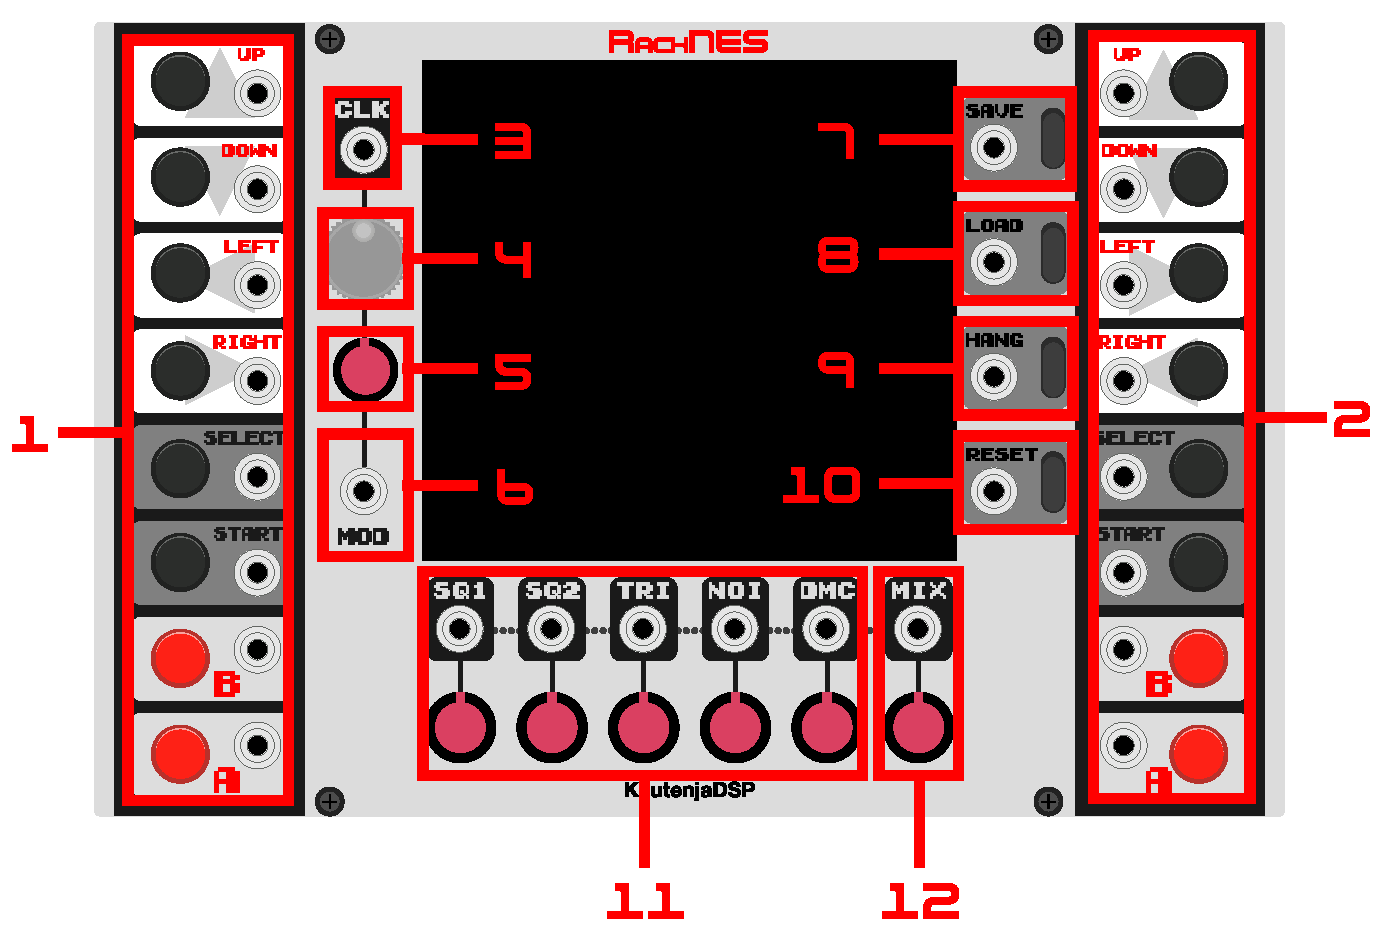
\includegraphics[width=\textwidth]{RackNES-Manual}
\clearpage

\begin{enumerate}
  \item Player 1 controller input triggers; high at $2V$
  \item Player 2 controller input triggers; high at $2V$
  \item NES Clock rate control. Controls the frame rate of the emulation from
    $2Hz$ to $1KHz$.
  \item NES Clock output. Pulse wave with $50\%$ duty cycle; high at $10V$,
    low at $0V$.
  \item NES Clock rate CV modulation. Modulates the clock rate parameter according
    to CV with half the range of the clock rate control knob.
  \item NES Clock rate CV attenuverter. Controls strength and polarity of
    clock rate CV input.
  \item Save state trigger; high at $2V$. Saves the current state of emulation.
  \item Load state trigger; high at $2V$. Loads the existing save state back
    into the emulation.
  \item Reset emulator trigger; high at $2V$. Equal to pressing "Reset" on the
    NES, resets the game.
  \item NES Audio output; $10V_{pp}$. Audio output from the internal mixer of
    the NES.
  \item NES Audio output volume level; $[0\%,200\%]$. Controls the gain of the
    audio output signal. $100\%$ is roughly $5V_{pp}$ and $200\%$ is roughly
    $10V_{pp}$ (though some clipping may occur).
\end{enumerate}

% References
% \nocite{*}
% \bibliographystyle{apalike}
% \bibliographies{literature}
\end{document}
